\documentclass[12pt]{article}

% basis equation commands
\usepackage{amssymb,amsmath}

% set 1 inch margins
\usepackage[margin=1.0in]{geometry}

% graphicx is needed for figures 
\usepackage{graphicx}

% natbib needed for citep and citet
\usepackage{natbib}

%set custom header and footer
\usepackage{fancyhdr} 
\pagestyle{fancy}

% name is on left, short title center, page on right
\lhead{Trever T. Hines}
\chead{RO 16-15 Reasearch Proposal}
\rhead{\thepage}
% get rid of page number in footer
\cfoot{}


%% Title
%%------------------------------------------------------------------------------
% make the title
\title{	
 \Large 
 % line bounding the title  
 \rule{\headwidth}{1.0pt}
 % left justify 
 \raggedright
 \textbf{Research proposal for RO 16-15:
 Novel crustal deformation models
 characterizing earthquake hazard and its uncertainties in the western U.S.}\
 % line bounding the title 
 \rule{\headwidth}{1.0pt} 
 % get rid of the date
 \date{}
 \vspace{-8ex}}

\begin{document} 
 \maketitle
 \thispagestyle{empty}
{\raggedright \large 
 \textbf{Trever T. Hines} \hfill\\
 \textbf{Advisor: Sarah Minson}\hfill\\
 \textbf{Location: Menlo Park}\hfill\\}

\section*{Research objective}
One of the goals identified in the USGS Natural Hazards Science Strategy is to assess natural hazards and to develop tools to improve upon those assessments.  An accurate assessment of seismic hazard requires estimates of where faults have previously ruptured as well as the uncertainties on those estimates.  The research proposed here addresses the latter.  The spatial extent of where a fault has slipped during an earthquake can be estimated from geodetic observations of ground deformation.  This is often an ill-posed problem because there may be many distributions of fault slip that are capable of describing the observed deformation. Of these candidate fault slip models, some may have magnitudes and directions of slip that are intuitively implausible.  Geodetic estimates of fault slip often include regularization in order to rule out these implausible models.  Regularization can be thought of as additional criteria that a fault slip model must satisfy.  For example, a preferred slip model may be required to vary smoothly over a fault in addition to adequately describing the observable surface deformation \citep[e.g.][]{Du1992}.  However, regularized estimates of fault slip lack meaningful quantifications of their uncertainty.  This is because uncertainties are highly dependent upon the choice of regularization, which is subjective and lacks physical justification.  Since the motivation behind adding regularization is to ensure that slip models are physically reasonable, the choice of regularization should be based on our understanding of how faults rupture.  From a Bayesian perspective, regularization that is physically motivated can be viewed as \textit{a priori} knowledge for inferences of fault slip.  The resulting \textit{a posteriori} estimate of fault slip would then be complete with a meaningful quantification of uncertainty.  My goal is to develop a Bayesian method for imposing physically motivated prior constraints on geodetic inferences of fault slip.  I then plan to apply this method to the 2004 Parkfield earthquake.  

\subsection*{Prior constraints on slip models}
I consider three well established, empirically derived relationships to use as prior constraints for slip models. (1) Faults slip in the direction of maximum shear stress \citep{Wallace1951}; (2) slip occurs when the Mohr-Coulomb failure criterion is exceeded \citep{Byerlee1978}; and (3) shear stress drop tends to be in the range of 0.1 to 10 MPa regardless of the spatial extent and magnitude of the earthquake \citep{Kanamori1975,Shearer2006}. I denote fault slip as $\Delta u$, shear stress as $\sigma_\parallel$, and shear stress drop as $\Delta \sigma_\parallel$, all of which are generally assumed to be spatially variable.  Constructing a prior based on the first two relationships would require an understanding of the background stress in the crust.  To constrain the direction of fault slip, only the orientation of the background stress needs to be known, which can be estimated from earthquake focal mechanisms.  The absolute background stress is necessary if I want to form a prior based on the Mohr-Coulomb failure criterion, which states that faults rupture when 
\begin{equation}\label{eq:MohrCoulomb}
  \mathbf{\sigma_\parallel} = C + \mu \mathbf{\sigma_\bot},
\end{equation}
where $\sigma_\bot$ is the normal stress on a fault, $C$ is cohesion, and $\mu$ is the coefficient of friction.  Barring earthquakes that produce significant stress overshoot, the shear stress drop at any point on a fault cannot exceed its frictional strength.  Additionally, the coseismic increase in shear stress along the edges of a rupture zone cannot exceed the frictional strength. In order to calculate the maximum shear stress for a strike-slip fault, I assume that the normal stress is primarily due to overburden.  Indirect inferences of the San Andreas fault strength which are based on heat flow and stress orientations across the fault find that $\mu\approx0.1$ \citep{Brune1969,Zoback1987}.  Laboratory experiments on gouge taken from the San Andreas fault find $\mu\approx0.3$ \citep{Carpenter2011}, and even higher values of 0.6 to 1.0 are suggested by \citet{Byerlee1978}. Even though the coefficient of friction can be debatable, I only need a reasonable upper bound on $\mu$ in order to limit the maximum shear stress drop in a slip model.  Assuming no cohesion and $\mu\approx0.3$, the shear stress required for an earthquake on a strike-slip fault is on the order of 100 MPa.  Therefore a slip model should satisfy the condition $|\Delta\sigma_\parallel|\lesssim 100$ MPa everywhere on a fault.  This can then be used to constrain $\Delta u$ through the relationship
\begin{equation}\label{eq:StressSlip}
  \Delta \sigma_\parallel (\xi_1) = \int_F K(\xi_1,\xi_2) \Delta u(\xi_2) d\xi_2,
\end{equation}
where $K(\xi_1,\xi_2)$ describes the stress drop at $\xi_1$ resulting from slip at $\xi_2$, and $F$ denotes the fault.  When assuming that the domain is a homogeneous, isotropic, elastic, half-space, $K$ can be computed with the analytical solution from \citet{Okada1992}.  

The observation that stress drop is consistently on the order of 0.1 to 10 MPa offers a tighter constraint on fault slip than the Mohr-Coulomb failure criterion.  Seismologically determined stress drops can be interpreted as the average coseismic change in shear stress over a rupture zone.  The difficulty is that the rupture zone is not known \textit{a priori} since that is what I am trying to estimate in a fault slip model.  However, it is known that stress drop is invariant to the spatial extent of the earthquake, and thus I can posit that the stress drop at each point on a ruptured fault should also be subject to the same bounds of 0.1 to 10 MPa.  Outside of the rupture zone, stress drop will generally be negative (i.e. pushed closer to failure).  When considering the entire fault, not just the area that ruptured, I can then impose an upper bound of 10 MPa on $\Delta \sigma_\parallel$.  \citet{Sun2011} also explored estimating fault slip with constraints on stress drop.  They assumed that stress drop must be uniform over the proposed fault geometry.  In contrast, I am merely imposing an upper limit on stress drop, which allows for greater flexibility in inferences of fault slip.        

\subsection*{Synthetic demonstration}
I use a synthetic test to demonstrate how effectively these physical constraints regularize fault slip models.  A thoroughly annotated IPython notebook containing all the work done for this synthetic test can be found in www.github.com/treverhines/ MendenhallProposal.git.  In this synthetic test, I calculate surface displacements resulting from slip on an infinitely long, strike-slip fault embedded in a homogeneous, elastic half-space.  This degenerates to a two-dimensional problem where the fault strike, fault slip, and displacements are in the anti-plane direction.  The fault extends from the surface to 15 km depth and is discretized into 10 segments. I impose fault slip that is consistent with a uniform stress drop of 5 MPa.  The slip and resulting displacements, with added noise, are shown in Figure 1.

I then use parameter estimation methods to attempt to recover the distribution of fault slip from the synthetic surface displacements while also imposing the above mentioned prior constraints. Estimating fault slip from surface displacements is typically done by solving 
\begin{equation}\label{eq:Forward}
  u(x) = \int_F G(x,\xi) \Delta u(\xi) d\xi
\end{equation}
for $\Delta u$ with linear least squares, where $u(x)$ are the observable coseismic surface displacements, and $G(x,\xi)$ describes displacements at $x$ resulting from slip on the fault at $\xi$.  For this synthetic test, my prior constraints are that $\Delta u$ is left-lateral, consistent with the orientation of maximum shear stress, and $\Delta \sigma_\parallel < 10$ MPa for each fault segment. I also add a prior constraint on the seismic potency, which I define for this two-dimensional problem as the average slip multiplied by the fault width.  I use a normally distributed prior for potency which has a mean of 0.6 $\mathrm{km}^2$ and standard deviation of 0.1 $\mathrm{km}^2$, while the potency for the true slip model is 0.58 $\mathrm{km}^2$. For the depths considered in this test, any reasonable value for the frictional strength of the fault would be greater than 10 MPa, and so there is no need to also include a friction-based prior. It is not possible to simultaneously impose all of the prior constraints considered here with the commonly used linear least squares or bounded value least squares methods.  I then resort to estimating $\Delta u$ with the more expensive, although more informative, Metropolis-Hastings algorithm, which is a Bayesian Monte Carlo method.  The Metropolis-Hastings algorithm randomly picks trial slip models and then determines the likelihood of each model based on how well they agree with the prior and how well they agree with the observed data. An ensemble of likely models are retained which represents the \textit{a posteriori} understanding of fault slip.  

\begin{figure}
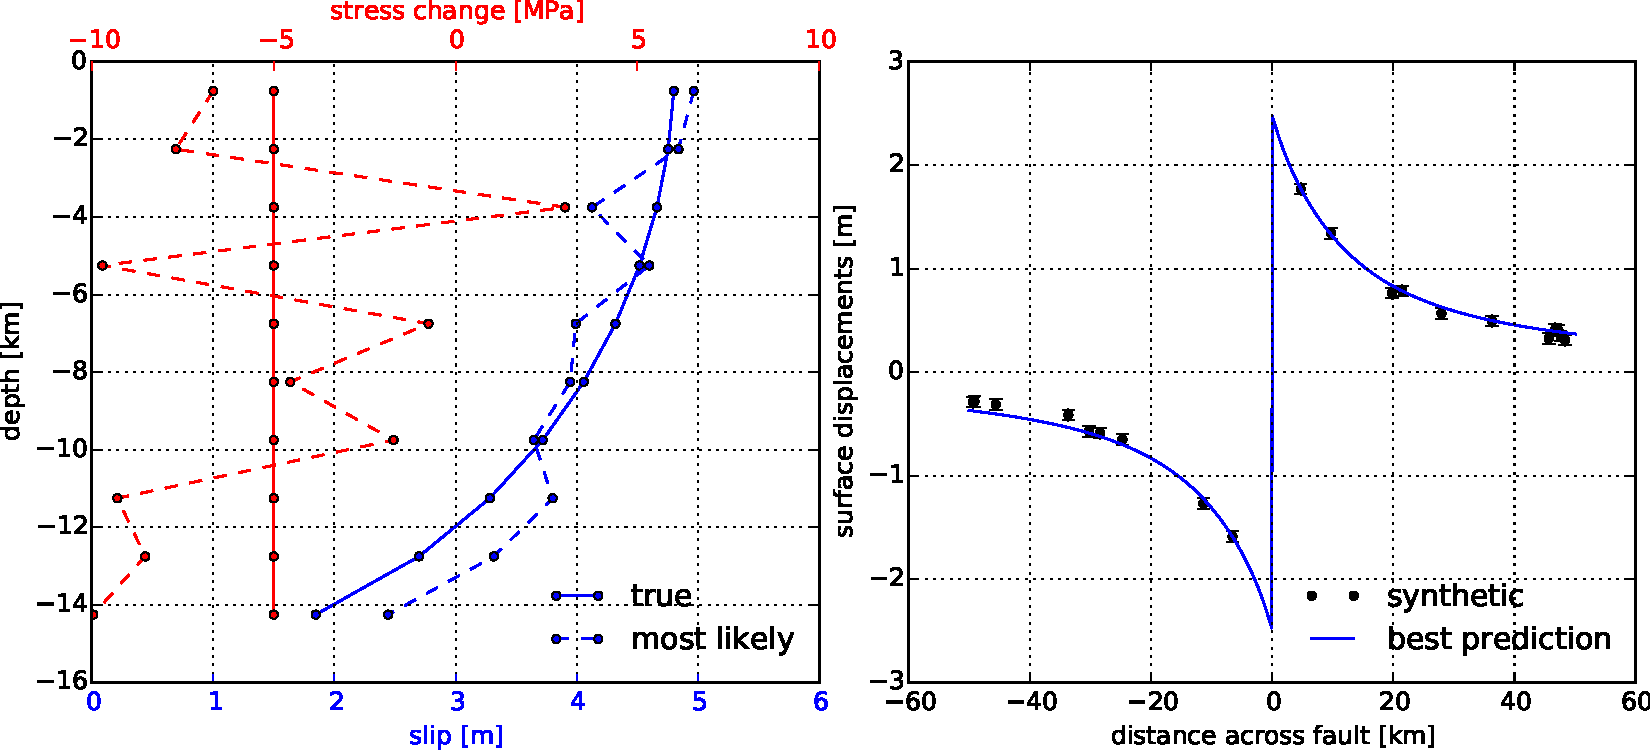
\includegraphics[width=1.0\textwidth]{figure_1}
\caption{Left: Left-lateral fault slip (solid blue) and corresponding stress change (solid red) used to generate the synthetic surface displacements. Note that a stress drop is a negative stress change.  Dashed blue and red lines indicate the slip and stress change, respectively, for the most likely posterior model. Right: Synthetic surface displacements (black dots) and surface displacements predicted by the most likely posterior model (blue).  Error bars on the synthetic displacements indicate one standard deviation of the added noise.}  
\end{figure}

I ran one million iterations of the Metropolis-Hastings algorithm, which takes about one minute on a desktop computer. The most likely slip model retained in the posterior is shown in Figure 1 along with the predicted displacements.  The most likely slip model closely resembles the true slip model; however, Figure 1 does not offer any information about the uncertainty in the inferred slip model. A great benefit to using a Bayesian Monte Carlo method is that we are able to view the distribution of likely fault slip models.  The left panel in Figure 2 shows the marginal posterior probability density functions of slip for each fault segment.  For comparison, I also used a Metropolis-Hastings algorithm to estimate fault slip but without a prior bound on stress drop.  The posterior distributions of slip with unbounded stress drop are shown in the right panel of Figure 2. When stress drop is unbounded, most of the retained models have no slip on all but a few fault segments, which then have 10s of meters of slip in order to produce the required potency.  As a result, the posterior slip distributions tend to be wide and have low mean values.  This is in sharp contrast to when stress drop is bounded.  In that case, the retained slip models vary smoothly with depth, and the marginal posteriors have mean values that closely match the true slip model.  This synthetic test demonstrates that physically motivated prior constraints can be used to effectively regularize an inference of fault slip while still retaining a meaningful quantification of uncertainty.  Moreover, introducing a prior constraint on stress drop reproduces the smoothness that is often sought when using standard regularization methods in inferences of fault slip.

\begin{figure}
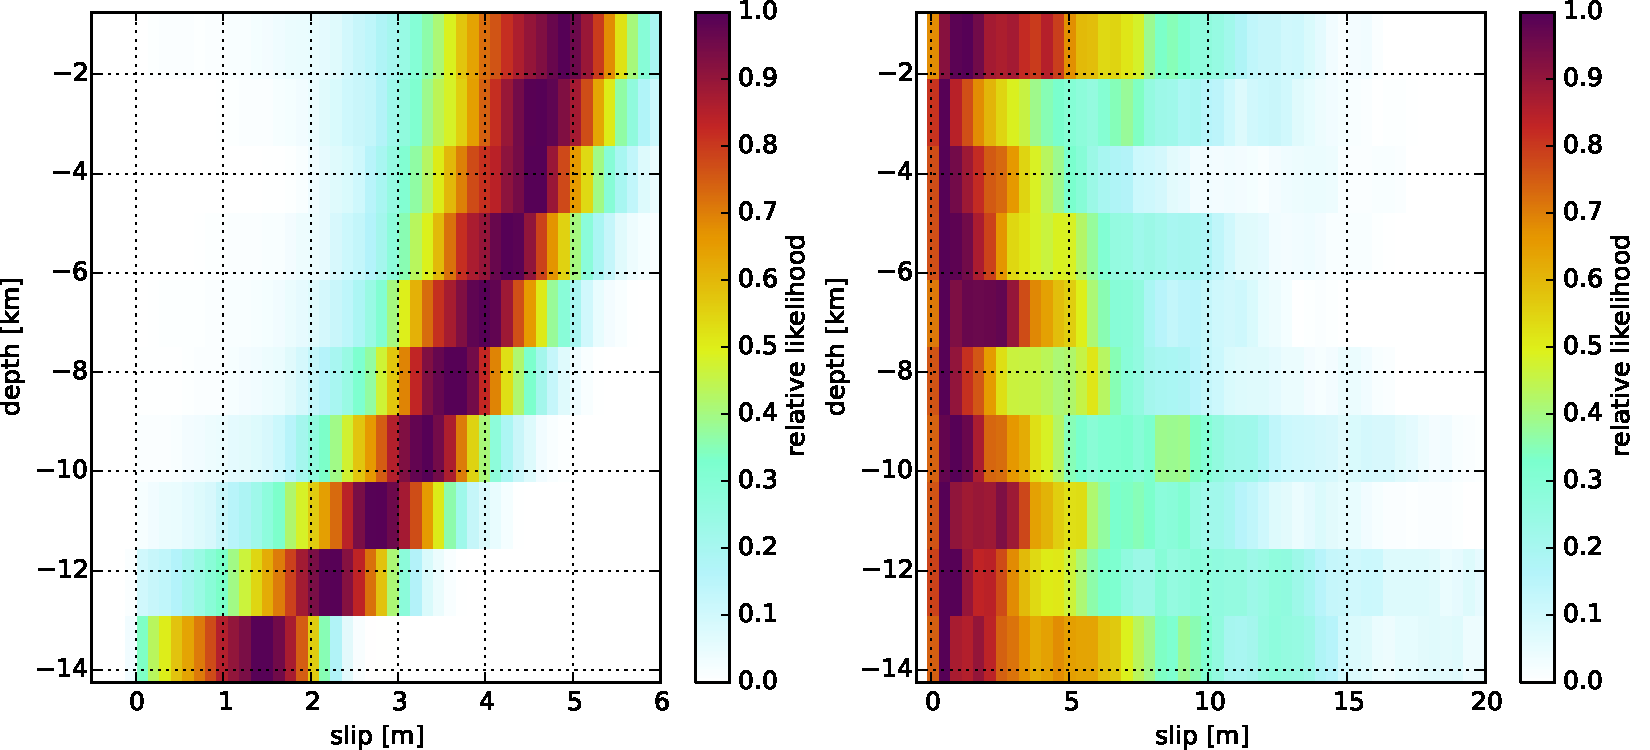
\includegraphics[width=1.0\textwidth]{figure_2}
\raggedleft
\caption{Marginal posterior probability density functions for slip on each of the discretized fault segments.  The left panel shows the PDFs when stress drop is bounded to be less than 10 MPa, and the right panel shows the PDFs when stress drop is unbounded.}  
\end{figure}

\subsection*{2004 Parkfield earthquake}
The 2004 Parkfield earthquake is an ideal testing ground for the above described Bayesian inference of fault slip.  One reason being that there is a wealth of data for this earthquake. Coseismic displacements were recorded by about a dozen ideally positioned, continuous GPS stations. InSAR and campaign GPS can also be used to estimated coseismic displacements although it is difficult to definitively discern coseismic from postseismic displacements for these data types \citep{Johanson2006}. Nonetheless, all of the data that I can potentially use to measure coseismic displacements have been made readily available through UNAVCO.  In addition to the wealth of geodetic data, the geometry of the Parkfield segment of the San Andreas fault is well known \citep{Simpson2006}.  This allows me to circumvent the computationally expensive task of trying to simultaneously estimate the fault geometry with the distribution of fault slip \citep[e.g.][]{Fukuda2008}. 

Revisiting the Parkfield earthquake from a Bayesian perspective could also have implications for assessing seismic hazard.  In particular, if we know where the San Andreas fault ruptured during the earthquake and we have a good understanding of the uncertainties on the slip model, then we can better quantify our confidence in where we believe slip deficits exist \citep{Murray2006}.  An accurate assessment of the location of slip deficits could then be used to improve existing seismic hazard models such as UCERF3 \citep{Field2014}.  Although \citet{Page2009} did attempt to quantify the uncertainty in slip models for Parkfield, their estimates of uncertainty were based on slip models with a smoothing regularization constraint making them difficult to interpret for the reasons mentioned above.

This project could also have implications for our understanding of afterslip.  The Parkfield earthquake was followed by a large amount of afterslip compared to the main shock \citep{Langbein2006,Johanson2006}.  It was noted, based on regularized slip models, that the spatial distribution of afterslip appeared to compliment the spatial distribution of coseismic slip.  However, without well quantified uncertainties on the inference of coseismic slip and afterslip, it is difficult to conclusively argue for such a spatial relationship. By inferring fault slip in a Bayesian sense with physically motivated priors, it will be possible to objectively assess whether afterslip is filling in regions that did not slip coseismically.  Understanding the relationship between coseismic slip and afterlip could then improve our understanding of fault friction.  Indeed, \citet{Johnson2006} and \citet{Barbot2009} have made inferences of the frictional properties of the Parkfield fault segment by modeling afterslip assuming that it is driven by coseismic stress change.  The coseismic stress changes in these studies came from geodetically derived estimates of coseismic slip.  The method of inferring coseismic fault slip described here could be a valuable tool for these kinds of studies because we explicitly force coseismic stress changes to be physically plausible, and thus predictions of subsequent afterslip would also be reasonable.  

\section*{Links to USGS science strategy}
This research fits in with two main aspects of the USGS Natural Hazards Science Strategy.  The first goal that this research addresses is to ``increase understanding of the underlying physical processes that produce hazard and determine where and under what conditions hazards occur".  This research answers ``where" hazards occur because a Bayesian inference of fault slip tells us the spatial extent of an earthquake and, most importantly, provides a meaningful quantification of uncertainty in that estimate.  Many existing geodetically derived models of fault slip lack any estimate of uncertainty, which makes them difficult to interpret and incorporate into assessments of seismic hazard. Thus this proposed research also aids in the USGS goal to ``create hazard assessments used to support decision making, based on fundamental understanding of natural hazards".

\section*{How and where research is to be conducted}
This research will be conducted at the USGS Menlo Park campus under the advisement of Sarah Minson.  The first stage of this project will be focused on further developing a method for inferring fault slip with physically motivated prior constraints.  With the success of the two-dimensional synthetic test, the next step will be to perform synthetic tests with more realistic, three-dimensional fault models.  This will introduce some geometric complexities that must be addressed.  For example, stress drop will be a vector quantity and the concept of an ``upper bound" on stress drop is not clearly defined.  Perhaps bounds could be imposed on the magnitude of stress drop or on stress drop along some direction.  I will need to run numerous synthetic tests to explore the effect of imposing various types of prior constraints on slip models.  An additional complexity is that three-dimensional slip models are discretized into a few hundred fault segments, meaning that the number of parameters being estimated will be far greater than the number of parameters estimated in my two-dimensional synthetic test. Inferring a large number of parameters will require implementing a more efficient algorithm than what was used here, such as CATMIP \citep{Minson2013}. 

The prior constraints on fault slip described in this proposal are only applicable to coseismic fault slip.  As mentioned, afterslip is a particularly significant deformation mechanism for the Parkfield earthquake. As part of the method developement, I would like to explore physically motivated prior constraints on afterslip.  For example, I can assume that afterslip results from the relaxation of coseismic stresses, and thus the stress drop resulting from afterslip cannot exceed the stress increases caused by coseismic slip.  Such a prior constraint on afterslip has been explored by \citet{Johnson2012}.  

The second stage for this project will be to apply this method to the 2004 Parkfield earthquake.  The continuous GPS data for this earthquake is available at UNAVCO and is ready to use.  The campaign GPS and InSAR data are also available through UNAVCO, although they are in their raw data format and need to be ran through processing software.  Once the data is compiled, performing a Bayesian estimation of fault slip should be straight forward.        

\section*{Required research facilities}
I will require a small cluster allocation with 10 to 100 CPUs to perform the computations for this research.  The Menlo Park campus has a cluster which would be sufficient for my computational requirements.  Additionally, I can apply for a cluster allocation through the Extreme Science and Engineering Discovery Environment (XSEDE).  If my XSEDE proposal is accepted then I will not require any USGS research facilities.  

Here I break down my estimate of computational requirements and verify that my proposed research is indeed tractable.  The Bayesian Monte Carlo algorithms used for this research can require a lot of computational resources because they involve testing many different slip models to see which are consistent with the observed data and the imposed prior constraints.  The number of models that need to be tested depends on the number of model parameters that are being estimated. Existing coseismic slip models for the 2004 Parkfield earthquake discretize the Parkfield segment of the San Andreas fault into about 300 patches. If slip is assumed to be entirely right-lateral then there are about 300 parameters that need to be estimated.  Based on the synthetic tests in \citet{Minson2013}, I would need to test about $10^{8}$ different slip models in order to adequately search a parameter space with that size.  The computation time then depends on how quickly each model can be tested.  If I have $N$ observations and $M$ unknown model parameters, then the computational cost of comparing the predictions of the trial model to the observed data is $O(NM)$.  The cost of testing if a trial model agrees with the prior is $O(M^2)$, where the main burden is in evaluating eq. (\ref{eq:StressSlip}) to ensure that stress drop is within the prior bounds.  However, the discretized matrix representing $K$ is sparse because stress drop on a fault segment is mostly a function of slip on nearby fault segments.  If I take advantage of this sparsity then the cost of comparing a test model to the prior is $O(M)$.  The main bottleneck in a Bayesian Monte Carlo algorithm is then comparing the observations to the predicted displacements for each trial model.  If I make a conservative estimate that this takes about one millisecond then the algorithm should finish in about one day on a single CPU.  Bayesian Monte Carlo algorithms are embarrassingly parallelizable and so the run time decreases linearly with the number of available CPUs.  I anticipate having to make numerous fault slip inferences for the purpose of synthetic testing and to explore various prior constraints.  If I have 10 to 100 CPUs available, then each inference would take about an hour to run, which I believe is sufficiently fast for my purposes.           

\newpage
\section*{Anticipated expenses}
I will need a desktop (${\sim}\$1,000$) for code development and small scale simulations.  For high performance computing needs, I will apply for a cluster allocation through the Extreme Science and Engineering Discovery Environment (XSEDE), which has no cost.  The only software that I will need, Python and Pylith \citep{Aagaard2013}, are free and open source.  Additional expenses will include travel for conferences (${\sim}\$3,000$) and publication fees (${\sim}\$2,000$). In total, I do not expect my research expenses to significantly exceed \$6,000.   



%\bibliography{mybib}{}
%\bibliographystyle{plain}
\bibliographystyle{apalike}
\bibliography{mybib}

\end{document}